\thispagestyle{plain}
\justifying

\begin{figure}
    \centering
    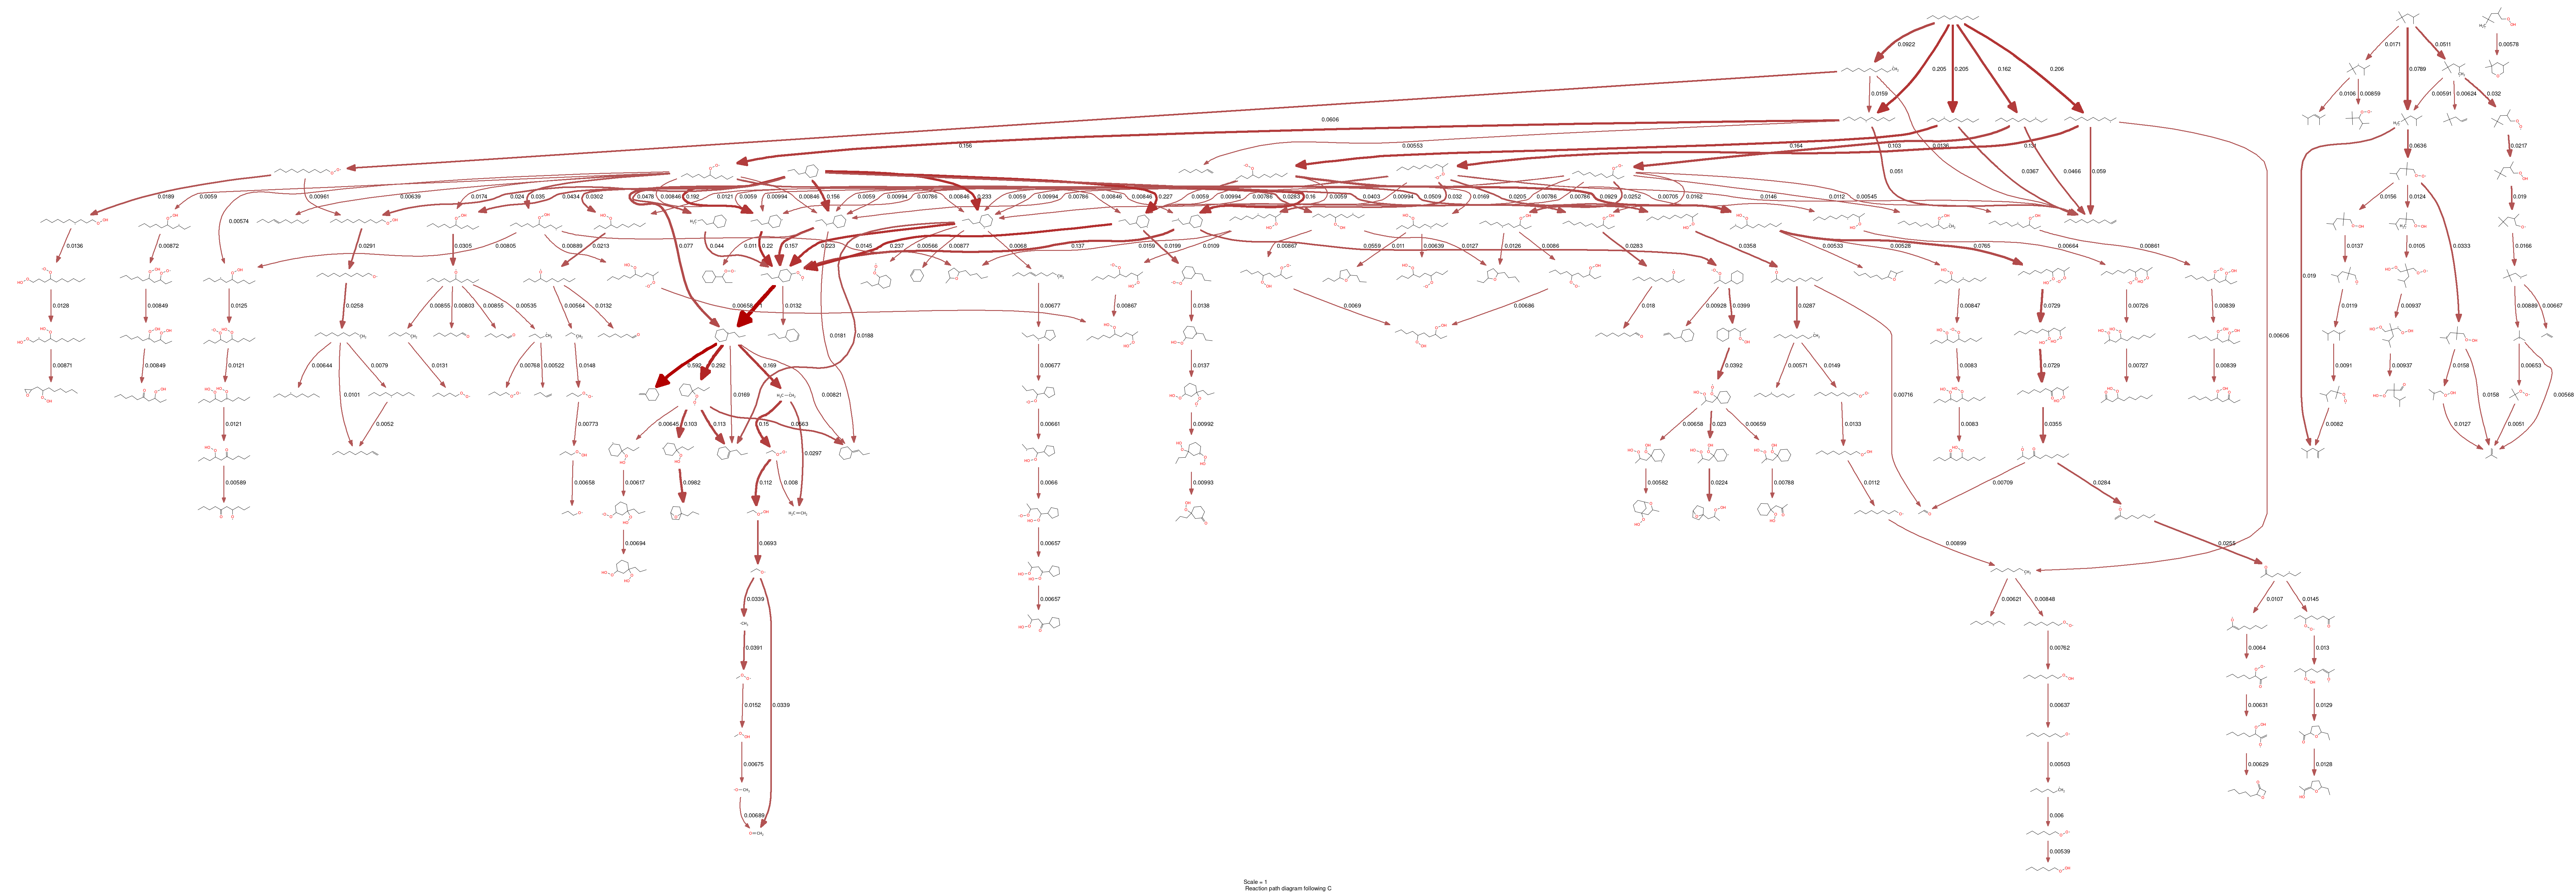
\includegraphics[scale=0.1, angle = 90, keepaspectratio]{images/GTL-PFA.png}
    \caption{Flux diagram of cross-reacted GTL fuel blend @ 900 K and 20 atm}
    \label{fig:gtl-pfa}
\end{figure}


\begin{figure}[ht]
     \centering
     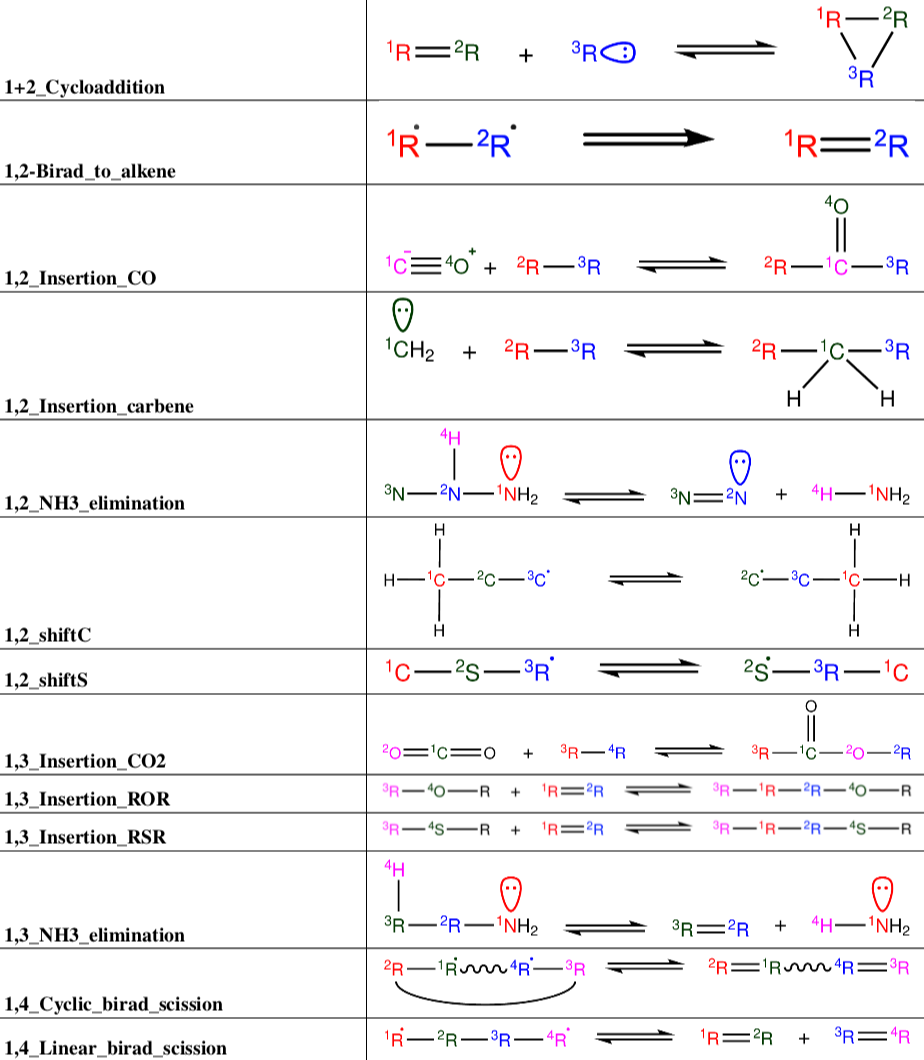
\includegraphics[scale=0.5, keepaspectratio]{images/rxn_fam1.png}
     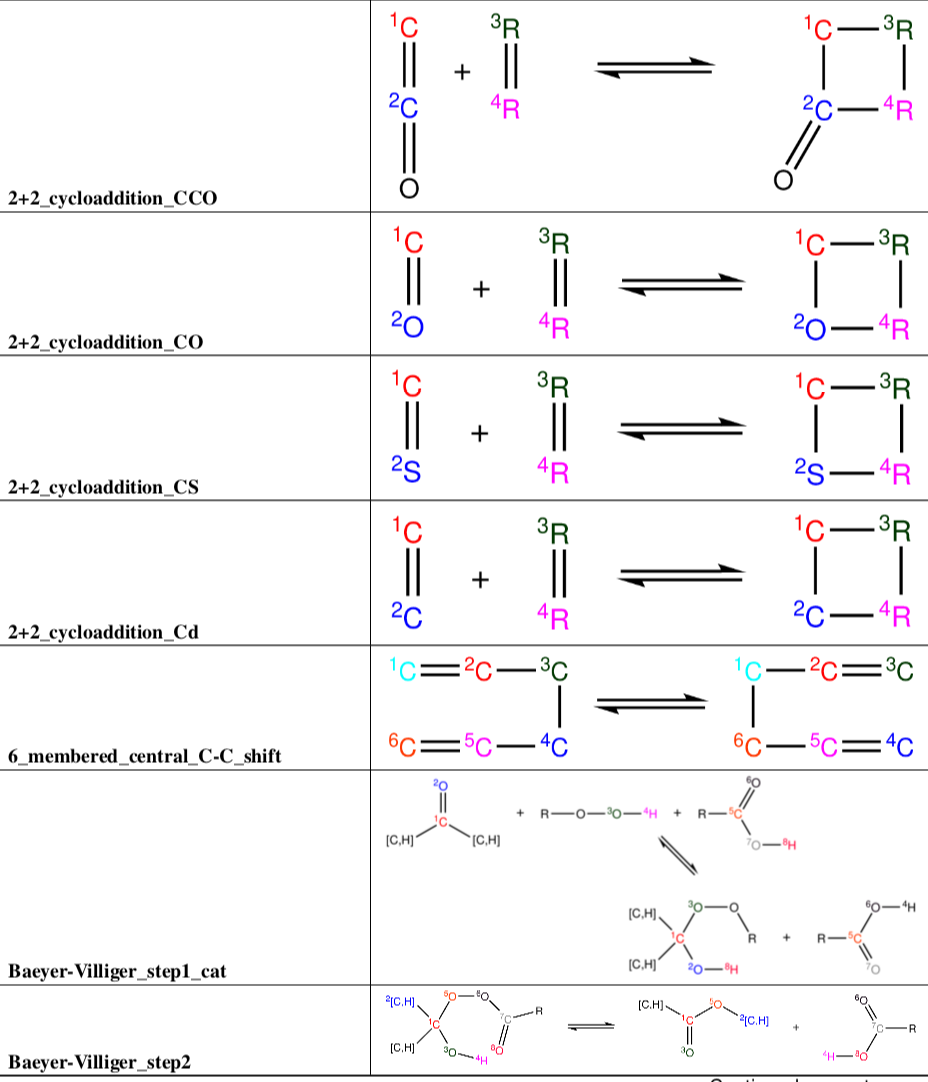
\includegraphics[scale=0.5, keepaspectratio]{images/rxn_fam2.png}
     \caption{RMG Reaction Families\cite{Gao2016ReactionMechanisms}}
     \label{fig:rxn_fam1}
 \end{figure}
 
 \begin{figure}
     \centering
     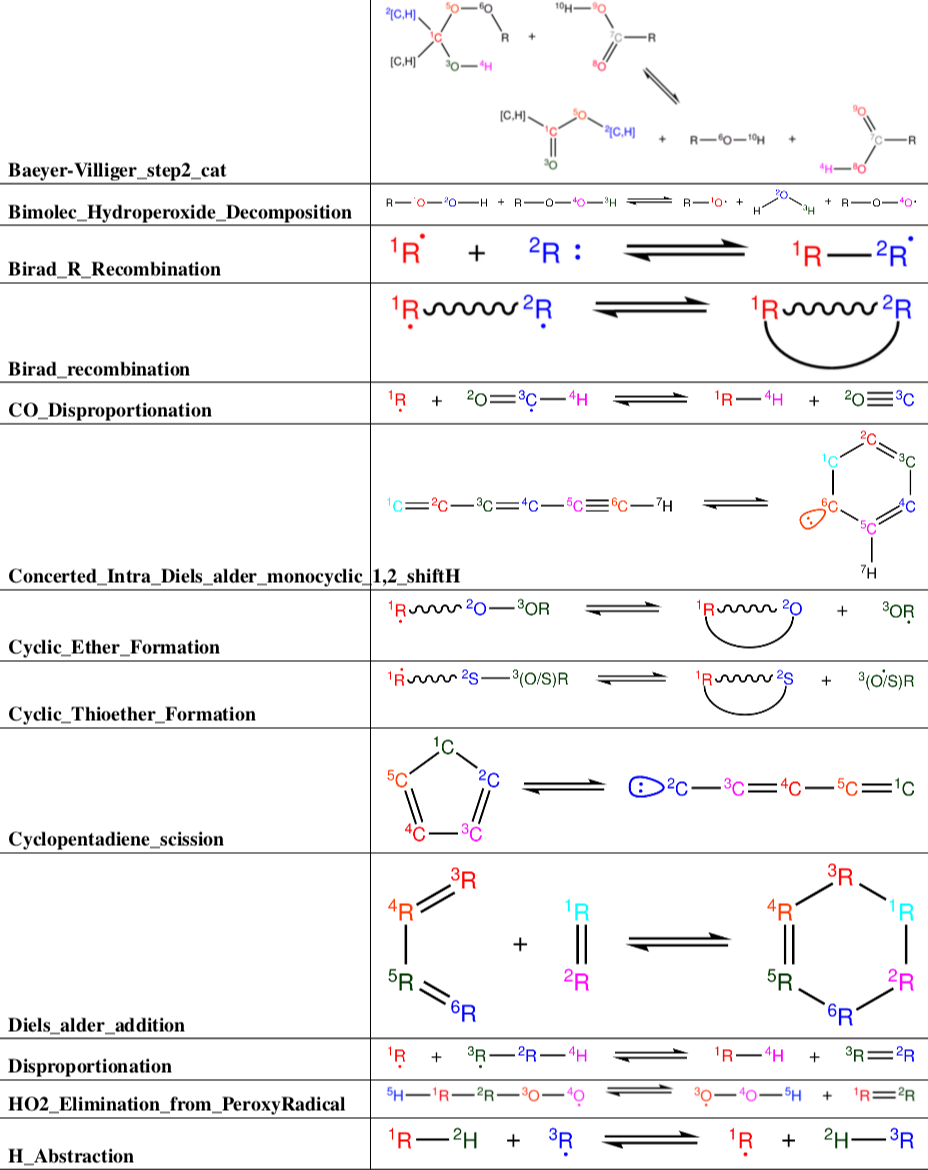
\includegraphics[scale=0.5, keepaspectratio]{images/rxn_fam3.png}
     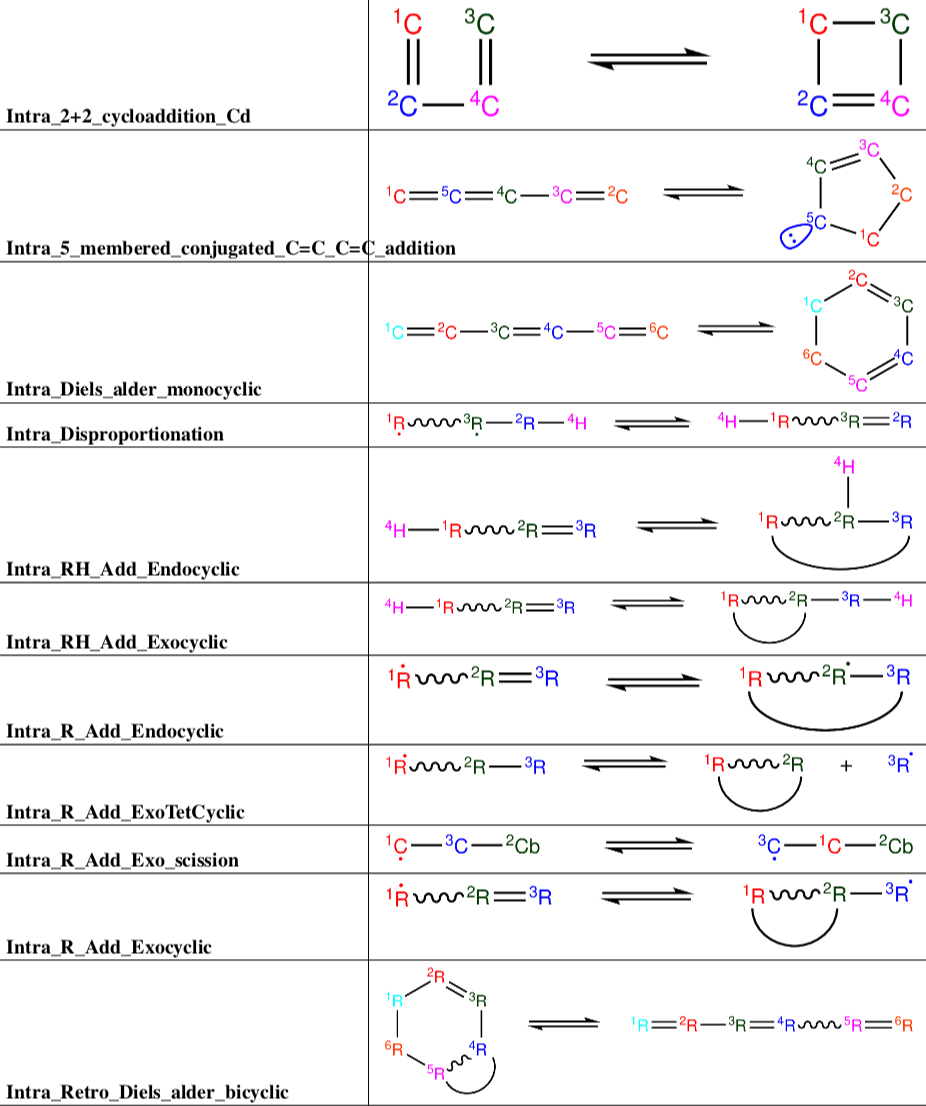
\includegraphics[scale=0.5, keepaspectratio]{images/rxn_fam4.png}
     \caption{RMG Reaction Families \cite{Gao2016ReactionMechanisms}}
     \label{fig:rxn_fam2}
 \end{figure}
 
 \begin{figure}
     \centering
     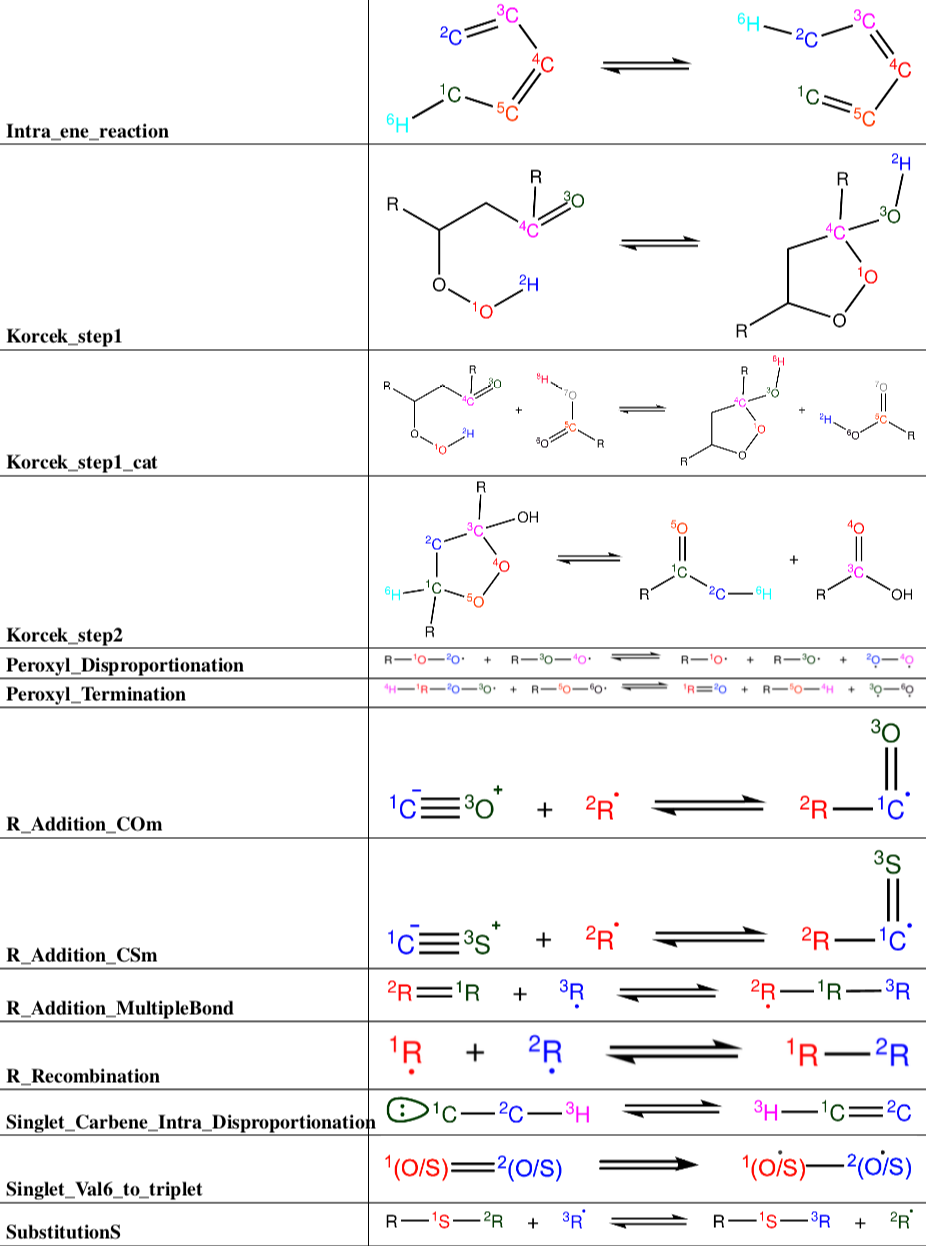
\includegraphics[scale=0.5, keepaspectratio]{images/rxn_fam5.png}
     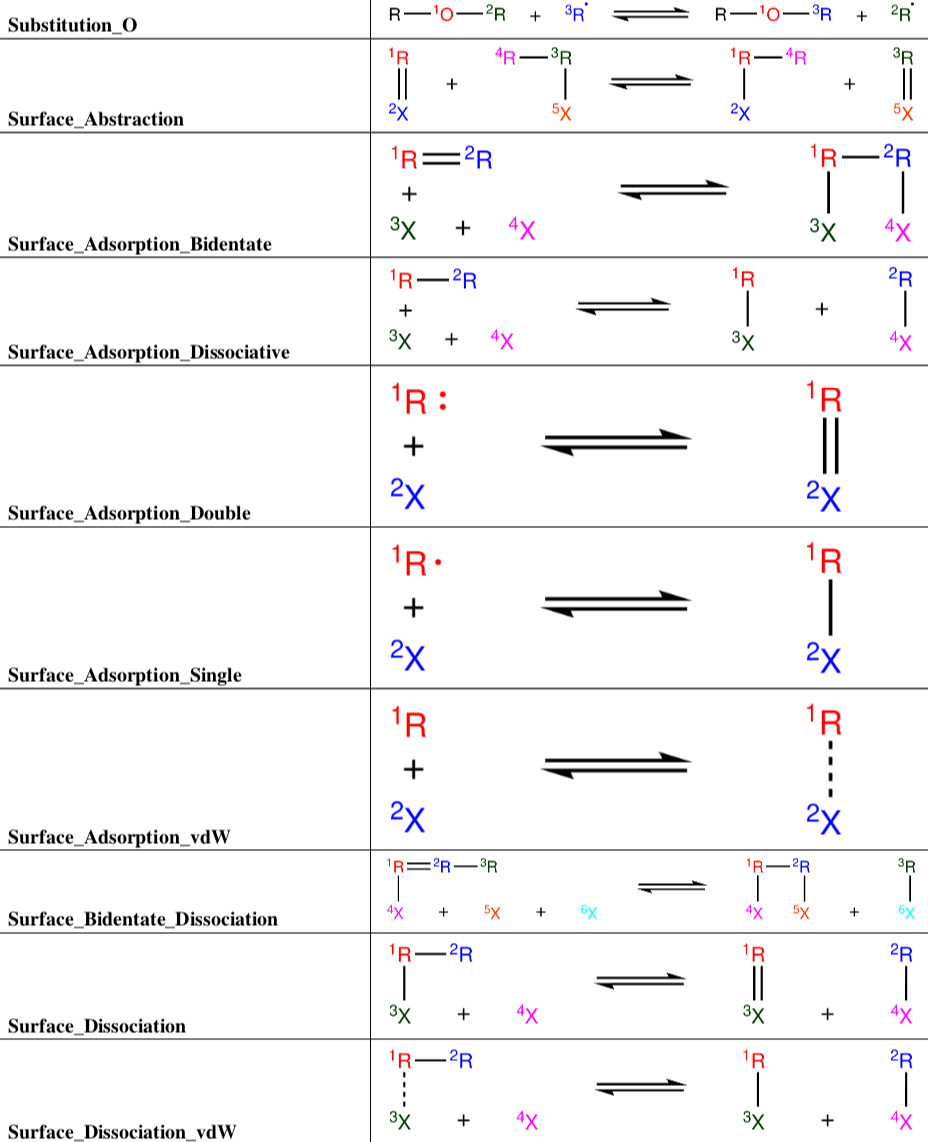
\includegraphics[scale=0.5, keepaspectratio]{images/rxn_fam6.png}
     \caption{RMG Reaction Families \cite{Gao2016ReactionMechanisms}}
     \label{fig:rxnfam3}
 \end{figure}
 \begin{figure}
     \centering
     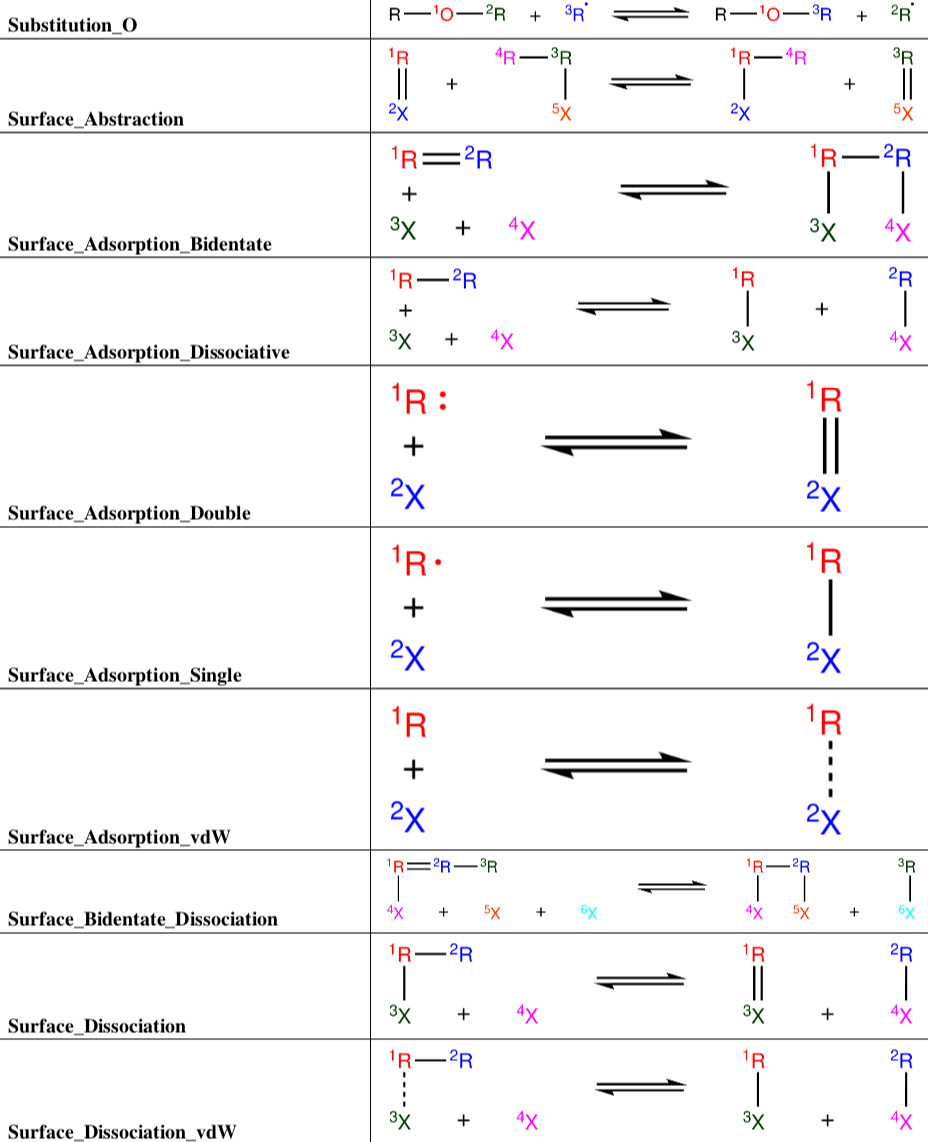
\includegraphics[scale=0.5, keepaspectratio]{images/rxn_fam6.png}
     \caption{RMG Reaction Families \cite{Gao2016ReactionMechanisms}}
     \label{fig:rxn_fam4}
 \end{figure}
 